\documentclass[czech,master]{resources/diploma/diploma}

% Sablonove baliky
\usepackage[autostyle=true,czech=quotes]{csquotes} % korektni sazba uvozovek, podpora pro balik biblatex
\usepackage[backend=biber, style=iso-numeric, alldates=iso]{biblatex} % bibliografie
\usepackage{dcolumn} % sloupce tabulky s ciselnymi hodnotami
\usepackage{subfig} % makra pro "podobrazky" a "podtabulky"

% Moje baliky
\usepackage{float} % lepsi umistovani obrazku (H)
\usepackage{glossaries} % balik pro praci s odbornymi pojmy
\usepackage{hyperref} % vkladani hypertextovych odkazu
\usepackage{xurl} % zalomeni dlouhych URL
\usepackage{tablefootnote} % poznámky pod tabulkou
\usepackage{color} % barvickyy
\usepackage{array} % schovavani sloupcu v tabulkach
\usepackage[linesnumbered,tworuled,vlined]{algorithm2e} % pseudokod
\usepackage{acro} % balík pro lepší práci s akronymy
\usepackage{svg} % pro vkládání SVG obrázků

% Pozadovane vstupy pro generovani titulnich stran.
\ThesisAuthor{Martin Korotwitschka}
\ThesisSupervisor{Ing. Jakub Beránek}

\CzechThesisTitle{Monitoring komplexních GitHub repozitářů}
\EnglishThesisTitle{Monitoring of Complex GitHub Repositories}

\SubmissionYear{2026}

\ThesisAssignmentFileName{../ThesisSpecification_KOR0289.pdf}

\Acknowledgement{%
Děkuji, že mám ještě tolik času na dokončení této práce.
}

\CzechAbstract{%
Abstract Ranalu
}
\CzechKeywords{git, github, rust, monitoring }

\EnglishAbstract{%
Abstract Ranalu but in english.
}
\EnglishKeywords{git, github, rust, monitoring }

% Acronym definitions using the `acro` package.
% Add `\usepackage{acro}` to your preamble (main.tex) if not already present.

\DeclareAcronym{vsb}{
	short = {VŠB},
	long  = {Vysoká škola Báňská}
}

\DeclareAcronym{vcs}{
	short = {VCS},
	long  = {Version Control System}
}

\DeclareAcronym{api}{
	short = {API},
	long  = {Application Programming Interface}
}

\DeclareAcronym{cli}{
	short = {CLI},
	long  = {Command Line Interface}
}

\DeclareAcronym{gui}{
	short = {GUI},
	long  = {Graphical User Interface}
}

\DeclareAcronym{ide}{
	short = {IDE},
	long  = {Integrated Development Environment}
}

\DeclareAcronym{http}{
	short = {HTTP},
	long  = {Hypertext Transfer Protocol}
}

\DeclareAcronym{ssh}{
	short = {SSH},
	long  = {Secure Shell}
}

\DeclareAcronym{url}{
	short = {URL},
	long  = {Uniform Resource Locator}
}

\DeclareAcronym{json}{
	short = {JSON},
	long  = {JavaScript Object Notation}
}

\DeclareAcronym{git}{
	short = {Git},
	long  = {Git}
}

\DeclareAcronym{svn}{
	short = {SVN},
	long  = {Subversion}
}

\DeclareAcronym{cvs}{
	short = {CVS},
	long  = {Concurrent Versions System}
}

\DeclareAcronym{sha}{
	short = {SHA},
	long  = {Secure Hash Algorithm}
}

\DeclareAcronym{tcpip}{
	short = {TCP/IP},
	long  = {Transmission Control Protocol/Internet Protocol}
}

\DeclareAcronym{https}{
	short = {HTTPS},
	long  = {Hypertext Transfer Protocol Secure}
}

% Shortcut macros: use `\API`, `\VSB`, etc. in your document.
\newcommand{\VSB}{\ac{vsb}}
\newcommand{\VCS}{\ac{vcs}}
\newcommand{\API}{\ac{api}}
\newcommand{\CLI}{\ac{cli}}
\newcommand{\GUI}{\ac{gui}}
\newcommand{\IDE}{\ac{ide}}
\newcommand{\HTTP}{\ac{http}}
\newcommand{\SSH}{\ac{ssh}}
\newcommand{\URL}{\ac{url}}
\newcommand{\JSON}{\ac{json}}
\newcommand{\GIT}{\ac{git}}
\newcommand{\SVN}{\ac{svn}}
\newcommand{\CVS}{\ac{cvs}}
\newcommand{\SHA}{\ac{sha}}
\newcommand{\TCPIP}{\ac{tcpip}}
\newcommand{\HTTPS}{\ac{https}}


\addbibresource{resources/sauce.bib}


% Minted things
\let\NewCommand\newcommand{}
% \immediate\write18{echo $ROAD > .ROAD.tex}
% \immediate\write18{echo $ROAD "nejhorší hack by žožka"}
% \input{.ROAD}
% \immediate\write18{export TEXMF_OUTPUT_DIRECTORY=\ROAD}


\usepackage{minted} %
\setminted{fontsize=\fontsize{9}{11}\selectfont, baselinestretch=1, frame=lines, framesep=8pt, linenos, breaklines}
\renewcommand\listingscaption{Výpis}
\renewcommand\listoflistingscaption{Seznam výpisů zdrojového kódu}

% Algorithm2e settings
% \DontPrintSemicolon
% \SetAlgoNoEnd
% \NoCaptionOfAlgo
% \SetKwProg{Fn}{Function}{:}{}
% \SetKwProg{return}{Return}{:}{}
% \SetKwData{True}{true}
% \SetKwData{False}{false}
% \SetKwFunction{FSwap}{Swap}
% \SetKwFunction{FLength}{Length}
% \newcommand{\bl}{\BlankLine}

% Uprava hloubky obsahu - pozdeji smazat !
\setcounter{tocdepth}{3}

% Custom reference
\newcommand{\customref}[2]{\hyperref[#2]{#1~\ref*{#2}}}
\newcommand{\chapterref}[1]{(\hyperref[#1]{Kapitola~\ref*{#1}})}
\newcommand{\imageref}[1]{(\hyperref[#1]{Obrázek~\ref*{#1}})}
\newcommand{\tableref}[1]{(\hyperref[#1]{Tabulka~\ref*{#1}})}
\newcommand{\listingref}[1]{(\hyperref[#1]{Výpis~\ref*{#1}})}
\newcommand{\glsref}[1]{\textit{\gls{#1}}}
\newcommand{\gameref}[1]{\textit{#1}}
\newcommand{\attr}[1]{(\texttt{#1})}
\newcommand{\devTool}[2]{\textit{#1}\footnote{\href{#2}{#2}}}

\newcommand{\todo}[1]{\noindent\textcolor{red}{TODO: #1}}

% Hide columns in tables
\newcolumntype{H}{>{\setbox0=\hbox\bgroup}c<{\egroup}@{}}


% Zacatek dokumentu
\begin{document}

% Titulni strany
\MakeTitlePages

% Seznam obrazku
\listoffigures
\clearpage

% Seznam tabulek
\listoftables
\clearpage

% Seznam výpisů zdrojového kódu
\addcontentsline{toc}{chapter}{Seznam výpisů zdrojového kódu}
\listoflistings
\clearpage

% Text
\chapter{Úvod}
\label{sec:Introduction}
Buckle up this will be speedrun of thesis on 400mg caffeine per day and 4 hours of sleep
\endinput


% - Verzování softwaru
%     - Verzování (co to je, jaké jsou systémy, hostované git služby)
%     - git (commity, repozitáře, větve, autoři commitů, modifikované soubory), struktura souborů na disku (bloby, git databáze), programovatelný přístup (libgit2 API)

\chapter{Versování}
\label{sec:versioning}
	Tato kapitola se bude věnovat versování a jeho významu pro vývoj a údržbu. Taktéž se bude věnovat konkrétnímu versovacímu nástroji git, jeho funkcím a jeho programovatelnému přístupu.

\section{Versování software}
	Versování je proces správy a sledování změn v projektu. V tomto procesu se uchovává historie veškerých změn v rámci souborů které jsou versovány. Nejšastěji se takovéto nástroje používají u textových zdrojových kodu softwaru. 

	Sytém správy verzí (VCS) \todo{aconym} obvykle eviduje kdo změnil jaký soubor a co konkrétního v tom souboru změnil. Díky tomu lze kdykoliv dohledat kdo napsal jakou část kodu případně proč byla tato část změněna. Proto u VCS lze ryhle vrátit zpět změny které by se ukázaly jako nevhodné.

	VCS řeší problém historie změn kdy před VCS bylo nutné uchovávat mnoho kopií téhož projektu s rúznými značkami o jakou verzi se jedná a to může vyžadovat nadměrně velkou disciplínu. Taktéž je vyžadováno o hodně více úložiště. U vcs často jsou ukládány pouze reálné změny oproti předchozí verzi a ne celá kopie projektu a jsou spravovány interně pouze VCS takže uživateli odpadne starost s organizací a ukládáním verzí.

	Další vlastností VCS je možnost pracování více uživatelů na stejných souborech. Vzhledem k tomu že VCS umožnuje řešit konflikty (takzvané merge konflikty) které vzniknou při změně stejného souboru více uživateli


	\begin{figure}[ht]
		\centering
		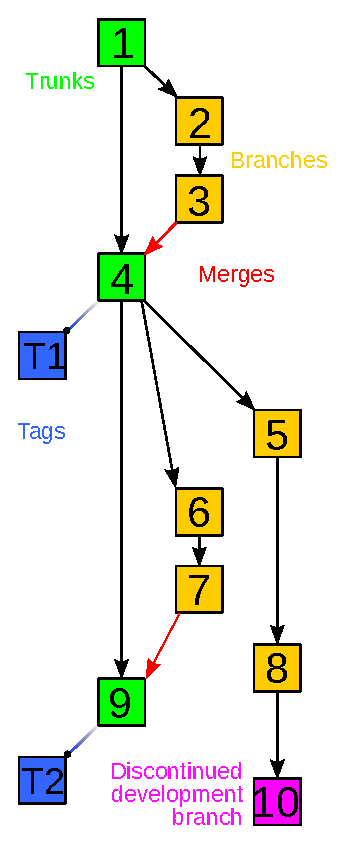
\includegraphics[height=\textwidth]{figures/vcs/Revision_controlled_project_visualization.pdf}
		\caption{Příklad historie projektu řízené verzovacím systémem.}
		\label{svg:revision_controlled_project_visualization}
	\end{figure}

	Základní ideální struktura v rámci grafu je lineární graf. tj řada bodů za sebou kde každá další vychází z té předchozí.
	Projekt má nějaký hlavní kořen (Trunk) \imageref{svg:revision_controlled_project_visualization} a z něj se poté větví ostatní větve (Branches) například pro vývoj nové funkcionality. Větve se poté slučují dokupy (Merges) a tím vznikají nové verze projektu. Z pohledu grafu se pak jedná o acyklický orientovaný graf. Samozřejmě může se ukázat že noě vyvíjená funkcionalita je nevyhovující a tak vzniká mrtvá větev (Discontnued development branch). Když už je kýžený počet změn v hlavní větvi tak se dělá tzv. tagování (Tags). Tag většinou ozačuje novou verzi projektu nebo označuje nějaký důležitý milník.

	\subsection{Centrální vs distribuované VCS}
	\label{sec:vcs}
		Hlavní rozdíl mezi centríálními a distribuovanými je v tom že distribuované VCS uchovávají historii jak u každého uživatele tak i na hostovací službě.

		U centrálního VCS se musí pouze spoléhat na hostovací službu a když ta vypadne tak v lepším případě uživatelé nemohou publikovat své změny a v horším případě se ztrácí historie pokud neexistují zálohy serveru. U distribuovaného VCS stačí aby nějaký z uživatelů měl projekt k dispozici protože každý uživatel co má projekt stažený má i dá se říci verzi zálohy s kompletní historií a jednoduše se může obnovit nebo znovu nasadit na jakoukoli jinou hostovací službu.

		Samozřejmě jsou rozdíly i k přístupu k repositáři. U centrálního VCS například příkaz \\ \code{svn commit} se aktualizujou přímo data na serveru zatím co u distribuovaného VCS (v tomtp řípadě gitu) příkaz \code{git commit} provede změny pouzev aktuálním lokálním repositáři. A až příkaz \code{git push} veškeré doteď commitnuté a nepropsané věci zapíše na hostovací službu. Tedy u centrálního VCS musíme být připojení k serveru pokud chceme publikovat změny zatímco u distribuovaného nemusíme. 

		Za zmínku stojí že příkaz \code{git pull} jsou dvě operace v jedné. Nejdříve se stáhnou změny ze serveru a poté se sloučí změny s lokálními změnami. Nejde tedy o opak k příkazu \code{git push}.

		\begin{figure}[]
			\centering
			\subfloat[Centralizované VCS]{\label{fig:centralized_vcs}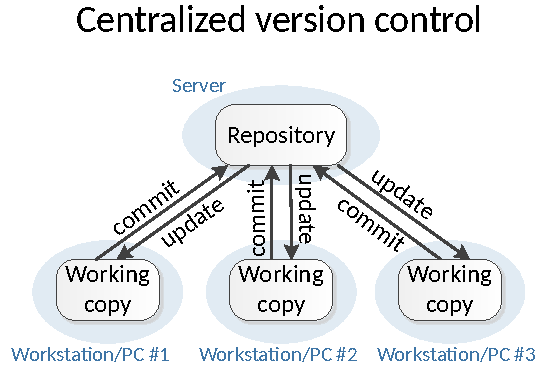
\includegraphics[width=0.45\textwidth]{figures/vcs/central-version-control.pdf}}
			\hfill
			\subfloat[Distribuované VCS]{\label{fig:distributed_vcs}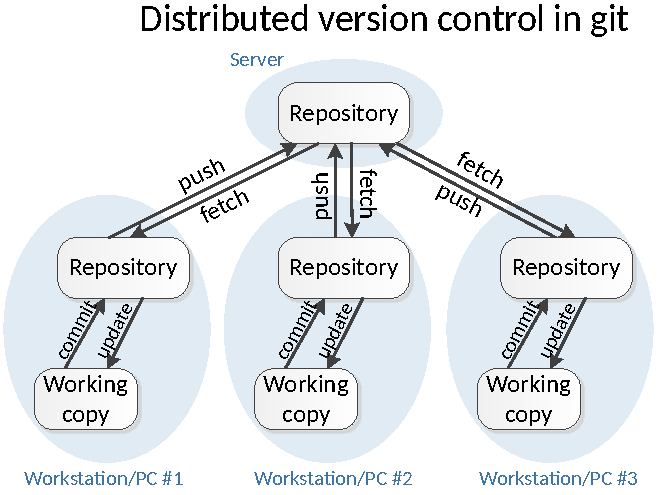
\includegraphics[width=0.45\textwidth]{figures/vcs/distributed-version-control.pdf}}
			\caption{Porovnání centralizované a distribuované architektury verzovacích systémů}
			\label{fig:vcs_comparison}
		\end{figure} 

		Rozdíl je i u toho jak se řeší konflikty a slučování větví. Centralizovaný VCS umožnuje provést aktualizaci ze serveru ikdyž uživatel má rozpracované neuložené soubory a systém automaticky smíchá všechny změny což může vést ke konfliktům. Distribuované VCS donutí uživatele nejdříve provést \code{commit}, tím se zapíšou změny od uživatele do historie a poté se může provést \code{merge} mezi dvěma pevnými body historie a vzniká nový pevný bod historie.



	\subsection{Apache Subversion}
	\label{sec:svn}
		Apache subversion (zkráceně SVN) je VCS, který vznikl v roce 2004 jako náhrada pro Concurrent Versioning System. Jendá se o open-source centralizovaný verzovací systém.

			Jeho hlavní implementační specifika jsou atomické revize a transakce, větvení za pomocí "Cheap copies", versování adresářů a metadat, podpora pro binární soubory, podpora neslučitelných soborů, a přístup k datům přes HTTP, HTTPS a SVN protokol.

			\subsubsection*{Globální revize a transakce}
			SVN používá globální revize napříč všemi soubory. U starších systémů byly nezávislé revize pouze pro daný soubor neboli každý soubor mměl svou historii a číslo revize. 

			Každý zápis do repositáře je atomický a je zapsán jako jedna revize napříč všemi soubory. To znamená že buď se zápis provede celý nebo se neprovede vůbec.
			Revize má jeden identifikátor který reprezentuje stav celého repositáře.

			\subsubsection*{Větvení za pomocí cheap copies}
			Větev v svn nemá v sobě žádnou pseciální reprezentaci větve. Větve jsou dělány na úrovni uživatelů pomocí adresářové struktury (tipicky /branches, /tags, /trunk).

			u větvení se kopíruje pomocí \code{svn copy}. Interně nedochází k fyzické duplikaci dat ale pouze se vytvoří symbolický odkaz na původní data v dané revizi. Tvorba nové větve nebo revize je tímto způsobem velice rychlá.

			\subsubsection*{Verzování adresářů a metadat}
			SVN odstranuje nedostatek ostatních sytémů které verzovaly pouze obsah a ne strukturu adresářů. 

			Přesuny, přejmenovávání a kopírování souborů je verzované a stále zachovávají návaznost na historii souboru. SVN taktéž umožnuje k adresáři připojit metadata ve formátu klíč:hodnota (např. \code{svn:ignore}, \code{svn:externals}). Tyto metadata jsou samozřejmě taky verzovaná stejně jako obsah souborů.


			\subsubsection*{Optimalizace pro jakékoliv soubory}
			Systém byl navržen tak že umí efektivně porovnávat i jakékoliv jiné soubory než jen textové. U binárních souborů se ukládají pouze změny oproti předchozí revizi a ne celá kopie souboru.  To jiným dřívějším souborům dělalo potíže.

			\subsubsection*{Podpora pro neslučitelné soubory}
			Při vývoji se může stát že pracujeme se soubory které algoritmicky sloučit nelze jako jsou například obrázky nebo zkompilované binární soubory. SVN umožnuje zamknout tyto soubory na púrovni serveru aby ostatní uživatelé je nemohli přepisovat dokud se tento zámek zase neuvolní.

			\subsubsection*{Přístup k datům}
			SVN nabízí flexibilní metoddy přístupu jak přes HTTP/HTTPS obohacené o verzovací funkce tak i přes vlastní svnserve protokol běžící nad tcpip a lehčí než http/https

	\subsection{Git}
	\label{sec:git}
		Git vychází z komerčního VCS BitKeeper, a zakládá si na několika klíčových požadavcích: 
		\begin{itemize}
			\item Rychlost
			\item Jednoduchý návrh
			\item Silná podpora nelineárního vývoje pro tisícovky paralelních větví
			\item Plně distribuovaný
			\item Schopnost efektivně spravovat velké projekty jako je kernel Linuxu
		\end{itemize}

		Oproti ostatním VCS které uchovávají historii jako seznam změn Git uchovává historii jako sérii snímků (snapshots). při každém commitu se uloží kompletní stav všech souborů a ne pouze změny. Když se v souboru oproti předchozímu snaphsotu nic nezměnilo tak se ukládá pouze odkaz na předchozí soubor. Tímto přístupem je docíleno efektivního větvení a slučování.

		V základu pracuje Git se třemi stavy souborů:
		\begin{itemize}
			\item Modifikované (modified) - soubor byl změněn a ještě se neuložil do historie
			\item Připravené (staged) - soubor je označen pro zarnutí do dalšího commitu
			\item Zapsané (committed) - změny jsou zaznamenány v historii
		\end{itemize}

		Z těchto stavů vyplývají i hlavní oblasti projektu na disku:
		\begin{itemize}
			\item Pracovní adresář (working directory) - obsahuje lokální kopii jedné verze projektu. Tyto soubory jsouvytaženy z lokální databáze git
			\item Oblast připravených změn (Staging area) - je soubor v kterém jsou uloženy informace o tom co bude obsahovat příští commit
			\item Adresář Git (Git directory) - obsahuje historii a metadata projektu
		\end{itemize}

		Mezi další specifika Gitu jsou že kromě distribuce dat na server a jejich synchonizace jsou všechny operace lokální. Tímto se dosahuje vysoké rychlosti a taktéž možnosti plně pracovat odkudkoliv bez nutnosti být připojen k síti. 

		Než se v gitu cokoliv uloží tak se nejdříve spočítá kontrolní součet (checksum) pomocí algoritmu SHA-1 který se pak používá k odkazování na uložená data. títo se zajistí že nelze provést jakoukoli operaci o které by git nevěděl a tím pádem data jsou vždy konzistentní.

		Když se v gitu provádí jakákoliv operace tak se data do databáze vždy přidávají. Samozřejmě lze systém přimět aby udělal něco co nelze vzít zpět ale je to obtížné. Samořejmě data lze poničit jako v jiných VCS ale když už jsou commitnuté tak se nedají ztratit. Díky tomu můžeme experimentovat a zkoušet různé věci bez starostí že něco ztratíme.

	\subsection{Programovatelný přístup k git}

\endinput
% - GitHub
%     - Jaké to má featury, jak vypadá contribution workflow, forky, PR, PR labely, CI workflows
%     - GitHub API (REST API, GraphQl, rate limity, autentizace, webhooky)

\chapter{GitHub}
\label{chap:github}
Tato kapitola se věnuje platformě GitHub, která je jedním z~nejpopulárnějších hostovaných řešení pro správu Git repozitářů. V~této kapitole budou popsány klíčové funkce GitHubu a~jeho \API{}.

% - GitHub
%     - Co je GitHub (hostovaná Git služba, největší platforma pro open-source vývoj)
%       - Stručná historie, jak vznikl, kdy byl odkoupen Microsoftem
%       - Jak se liší od prostého gitu (sociální funkce, webové rozhraní, CI/CD, Issues, wiki...)

\section{Úvod do GitHubu}
\label{sec:github_introduction}
GitHub je jedna z~mnoha hostovaných služeb pro správu Git repozitářů. Rozšiřuje základní funkcionalitu Gitu o~sociální funkce, webové rozhraní, \CICD a~další.
Nejznámější alternativy jsou \devTool{GitLab}{https://gitlab.com}, který je na rozdíl od GitHubu open-source a~umožňuje vlastní provoz (self-hosting), a~\devTool{Bitbucket}{https://bitbucket.org}~\cite{psl_git_tutorial_main}.

Po vzniku Gitu pro jádro operačního systému Linux se brzy ukázalo, že vlastní hostování repozitářů není vždy dostačující a~vznikla poptávka po sdílené cloudové službě. V~roce 2008 proto vznikl GitHub a~od té doby se stal největší platformou pro open-source vývoj. V~roce 2018 byl odkoupen společností Microsoft~\cite{psl_git_tutorial_main}.

Hlavní rozdíl mezi Gitem a~GitHubem spočívá v~tom, že Git je nástroj pro správu verzí (\VCS), zatímco GitHub je kompletní vývojová platforma. Kromě samotného Gitu nabízí možnosti \CICD a~nasazení, sledování chyb a~požadavků (issue tracking), správu pull requestů, diskuzní fóra komunity a~další sociální funkce. GitHub také umožňuje hostování statických stránek prostřednictvím služby \devTool{GitHub Pages}{https://pages.github.com}, která se využívá například pro hostování dokumentace projektů. Samozřejmostí je webové rozhraní pro veškerou správu včetně úpravy kódu a~kontroly pull requestů.

% - Základní funkce a model spolupráce
%   - Repozitáře (veřejné / soukromé, forky)
%     - Fork: kopie repozitáře pod jiným uživatelem, smysl pro přispívání do cizích projektů
%     - Hvězdičky, watchers
%   - Issues
%     - Sledování chyb a požadavků na funkce
%     - Labely (kategorizace, prioritizace), milníky, přiřazení
%   - Pull Requesty (PR)
%     - Contribution workflow: fork → větev → commit → PR → review → merge
%     - Review proces: review komentáře, schvalování, požadované změny
%     - Labely na PR (stejný systém jako Issues)
%     - Draft PR, auto-merge
%     - Propojení PR s Issues (closing keywords: "Closes #123")
%   - GitHub Actions (CI/CD)
%     - Workflow soubory v .github/workflows/ (YAML)
%     - Triggery (push, PR, schedule, workflow_dispatch...)
%     - Runners (GitHub-hosted vs. self-hosted)
%     - Využití v kontextu monitoringu: automatické spouštění aktualizací dat
%   - Projekty a milníky (GitHub Projects)
% - GitHub API
%   - REST API
%     - Základní vlastnosti: HTTP, JSON, verzování (v3)
%     - Autentizace: Personal Access Token (PAT), GitHub App, OAuth
%     - Příklady endpointů relevantních pro monitoring (issues, PRs, commits, labels...)
%   - GraphQL API (v4)
%     - Motivace: REST vracelo příliš mnoho/málo dat, GraphQL umožňuje dotaz na přesně požadovaná pole
%     - Základní syntaxe dotazu, ukázka
%     - Výhody pro monitoring velkých repozitářů (méně requestů, přesnější data)
%     - Omezení API (rychlost)
%   - Rate limiting
%     - REST: 5 000 requestů/hod pro autentizované uživatele
%     - GraphQL: bodový systém (cost/complexity)
%     - Hlavičky X-RateLimit-*, strategie pro vyhnutí se limitům (throttling, caching)
%   - Webhooky
%     - Push notifikace při události (PR otevřen/zavřen, push, label přidán...)
%     - Alternativa k polling přístupu, výhody a nevýhody
%     - Typy eventů relevantních pro monitoring
\input{./chapters/theory/existing_tools.tex}
\input{./chapters/theory/used_technologies.tex}
\input{./chapters/theory/rust_repository.tex}

\input{./chapters/implementation/design.tex}
\input{./chapters/implementation/implementation.tex}
\input{./chapters/implementation/evaluation.tex}


\chapter{Závěr}
Chtěl bych poděkovat všem že jsem z toho nezešílel
a fsamozřejmě všechny požadavky byly splněny jak jinak že ano
\endinput

% Seznam literatury
\printbibliography[title={Literatura}, heading=bibintoc]

% Přílohy
\appendix

\end{document}
